\subsection{Executed first-entry mechanism study}

The executed mechanism study contains 20 fresh markets from seeds 40001--40020, using $N=500$, $p=100$ and the 15-year DGP of the baseline. The four arms share every candidate shadow policy and every realized utility score. All 100 comparisons remain under observation to the common horizon, including after crossing. These are fixed-reference mechanism experiments, not twenty new full-strategy backtests.

\begin{table}[H]\centering\small

\begin{tabular}{lrrrr}

\toprule

Arm & Entry markets & Before end & Median year & Max. log E \\

\midrule

Catoni--baseline & 0/20 & 0/20 & NA & 0.008 \\

Catoni--geometry & 0/20 & 0/20 & NA & 0.555 \\

Tail--uniform & 0/20 & 0/20 & NA & 0.710 \\

Tail--geometry & 19/20 & 18/20 & 12.0 & 4.918 \\

\bottomrule\end{tabular}

\caption{Annual eligible first-entry events. ``Before end'' excludes a first crossing at the terminal revision. Median year is conditional on crossing; censored markets remain in the entry-rate denominator. No actual post-entry fund path is simulated.}\end{table}

The corrected-tail geometric arm has 19 entry markets out of 20; the Wilson 95\% interval for this market-level fraction is [0.764, 0.991]. It is a search outcome over 100 candidates, not an individual-test power estimate or a globally controlled rejection probability. One first certification occurs only at the terminal revision; 18 markets have any remaining market observations after certification. Neither geometric Catoni nor uniform-moment corrected-tail betting alone produces an entry in these 20 markets. The combined change improves statistical feasibility but does not remove the substantial cost of waiting.

4 selected first policies use structural proxies whose own coefficient is fixed at zero in the generator. Their conditional shadow gains are positive on the last evaluated date before selection. This illustrates the distinction between structural and economic relevance; it is not a false-discovery calibration result. These conditional gains refer to the shadow state, not a claim that the fund can acquire the shadow positions without paying its actual entry cost.

An additional post-hoc action audit replays all selected histories, refits with then-available observations and computes a hypothetical next-period entry from the fund's actual zero allocation. It values that action with true current model moments after selection, without drawing the next return. 18 of 18 nonterminal entries have positive conditional utility after actual entry costs. The mean is 0.957 basis points of daily utility, compared with 2.457 for the continuing shadow; the actual entry cost is 1.500 basis points. This conditional action valuation is descriptive and supplies no post-entry fund path or new guarantee of current profitability.

Separate predictable skew-null diagnostics use 10,000 independent paths and 2,000 observations. The corrected mixture crosses at rate 0.0068 (Wilson interval [0.0054, 0.0086]). An invalid single bettor ($B_t=V_{4,t}^{1/4}$, fraction $.75$) without bias correction crosses at rate 0.9966. This is an invalidity demonstration; its configuration differs from the mixture, so it is not a matched power comparison.

\begin{figure}[H]\centering

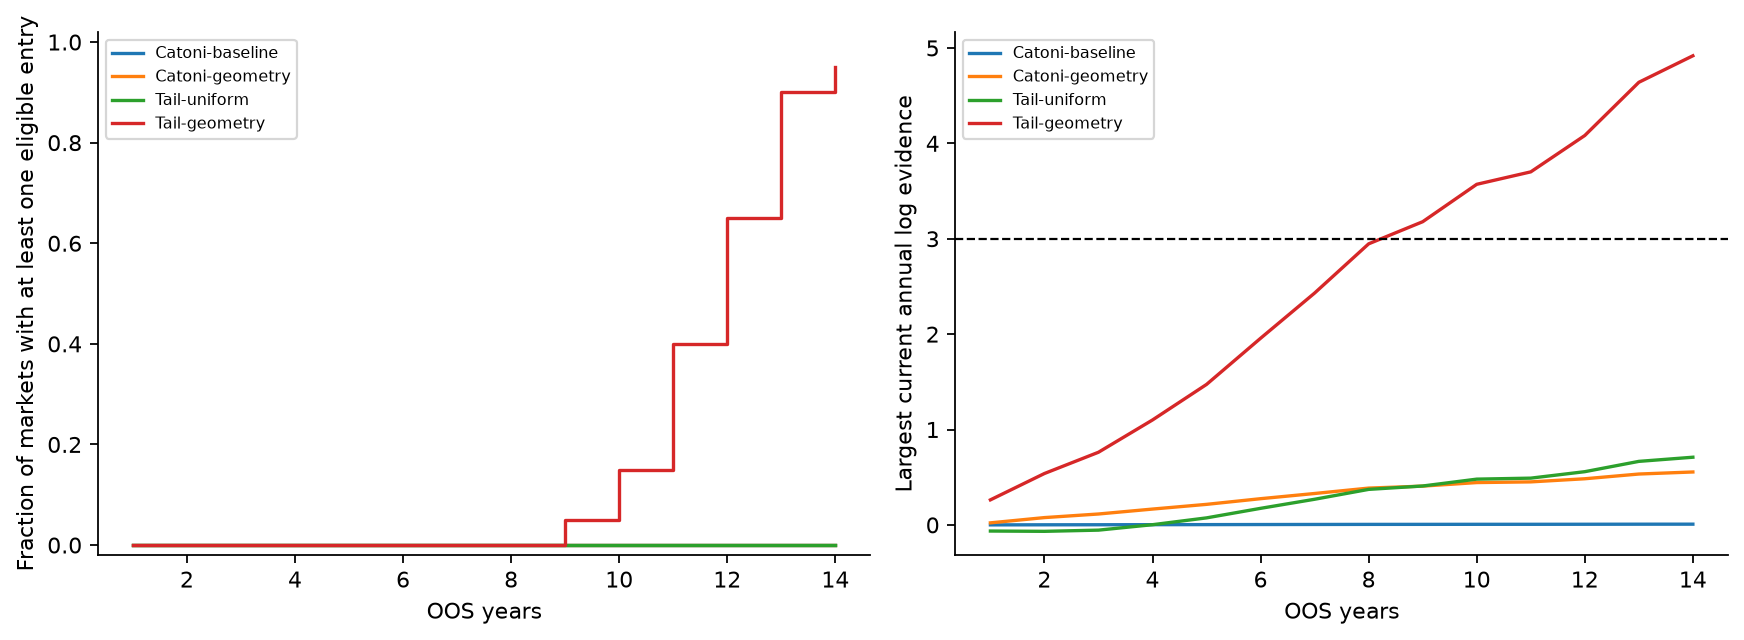
\includegraphics[width=.97\linewidth]{figures/first_entry_feasibility.png}

\caption{First-entry feasibility across twenty complete fresh markets. Every arm uses the same scores. Curves include terminal test events, with no claim of post-entry trading performance.}

\end{figure}

\begin{figure}[H]\centering

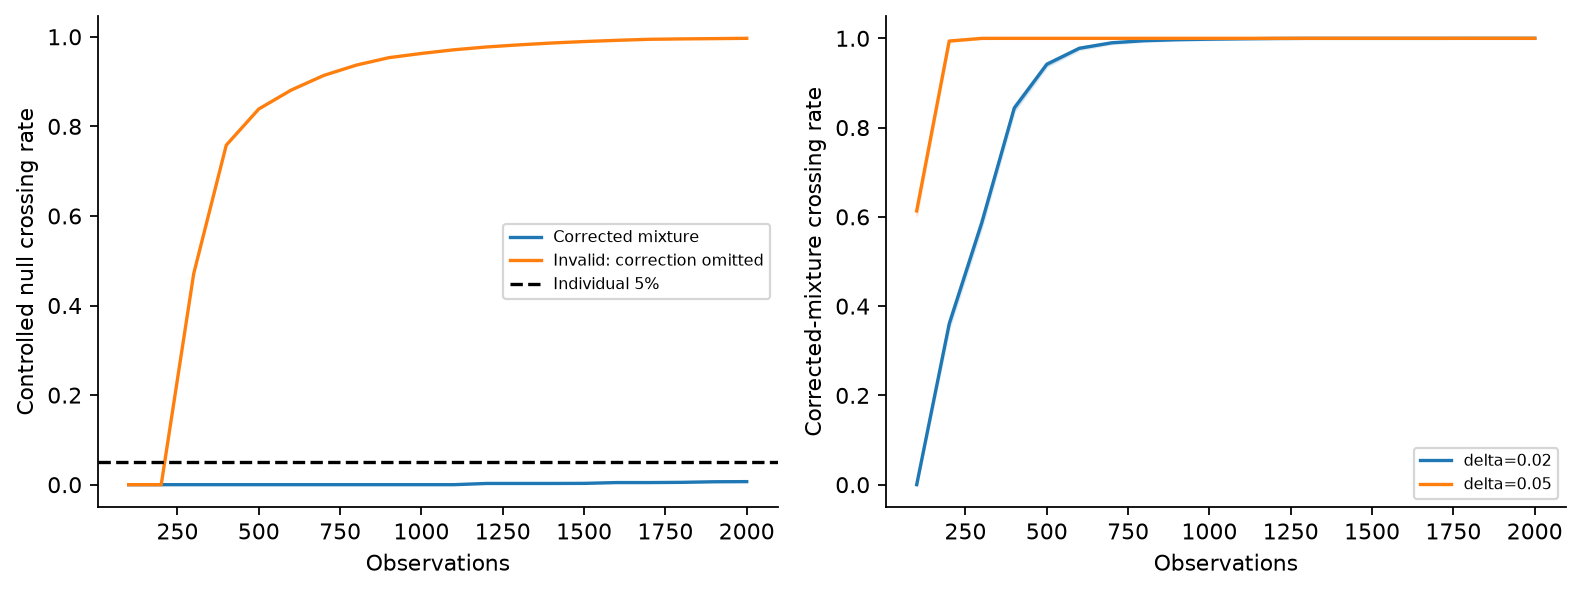
\includegraphics[width=.97\linewidth]{figures/controlled_tail_calibration.png}

\caption{Controlled statistical experiment under a predictable skewed null and two positive-mean alternatives. The invalid negative control is a single uncorrected bettor; it is not a matched power comparison with the corrected mixture. Shading shows Wilson intervals across independent paths.}

\end{figure}

\FloatBarrier
